\documentclass{article}

% if you need to pass options to natbib, use, e.g.:
%     \PassOptionsToPackage{numbers, compress}{natbib}
% before loading neurips_2021

% ready for submission
\usepackage[final]{neurips_2021}
% to compile a preprint version, e.g., for submission to arXiv, add add the
% [preprint] option:
%     \usepackage[preprint]{neurips_2021}

% to compile a camera-ready version, add the [final] option, e.g.:
%     \usepackage[final]{neurips_2021}

% to avoid loading the natbib package, add option nonatbib:
%    \usepackage[nonatbib]{neurips_2021}

\usepackage[utf8]{inputenc} % allow utf-8 input
\usepackage[T1]{fontenc}    % use 8-bit T1 fonts
\usepackage{hyperref}       % hyperlinks
\usepackage{url}            % simple URL typesetting
\usepackage{booktabs}       % professional-quality tables
\usepackage{amsfonts}       % blackboard math symbols
\usepackage{nicefrac}       % compact symbols for 1/2, etc.
\usepackage{microtype}      % microtypography
\usepackage{xcolor}         % colors
\usepackage{graphicx}		% image inserting

\title{Project Proposal 8420}

% The \author macro works with any number of authors. There are two commands
% used to separate the names and addresses of multiple authors: \And and \AND.
%
% Using \And between authors leaves it to LaTeX to determine where to break the
% lines. Using \AND forces a line break at that point. So, if LaTeX puts 3 of 4
% authors names on the first line, and the last on the second line, try using
% \AND instead of \And before the third author name.

\author{%
	Will Sherrer \\
	Clemson University\\
	wsherre@g.clemson.edu \\
	\And Ashton Sobeck \\
	Clemson University\\
	asobeck@g.clemson.edu
}





\begin{document}
\maketitle
%\section{Submission of papers to NeurIPS 2021}
\section{Abstract} 

Our group explores the effectiveness of Convolutional Neural Networks (CNN) 
  when  images that have been reduced by Principal Component Analysis (PCA) have 
  been input as training.  We use the Canadian Institute for Advanced 
  Research (CIFAR) dataset to conduct PCA on and compare how different amount of 
  features in input images effect the accuracy of a CNN.

\section{Motivation}

Throughout our class of CPSC 8420, we have learned many things. 
One of the most crucial concepts of the class is certainly Singluar Value 
Decomposition (SVD). Using SVD, one can utilize PCA to find the important 
features of data. CNNs are quite effective in identifying patterns within 
images through the use of filters and non-linearity within their structure. 
However, when input images get larger and larger, the network can grow in 
size and in return, require much more computational power to train in a timely manner.

\section{Method}

The machine learning techniques we plan to implement are PCA and SVD. These will be used to reduce the dimension of an images which the CNN models will be trained and tested on. A technique we could be improving on is seeing if CNN models can maintain performance whilst minimizing input data. We believe this could be a good preliminary study on performance vs. training sample data. 

\section{Experiment Overview}

The experiment that we conducted is using 2 CNN models with different architectures. Having two models will just test if one architecture is better than another with testing. We then take the CIFAR10 dataset images and train the models with the original image as a control. We record the training loss and accuracy as well as testing loss and accuracy. Then, we use PCA to reduce the data further to 3.125\%, 6.125\%, 12.5\%, and 18.75\% of the original and train both models with the same hyper-parameters for consistency. We record the training and testing loss and accuracy and plot the data and compare to see if the models are able to learn a reduced image. 

\section{Related Research}

We found an interesting paper, "Image retrieval method based on CNN and
dimension reduction" (https://arxiv.org/pdf/1901.03924.pdf) that also conducts a study on this topic. They found that while CNN's can still have satisfactory performance, further practical and theoretical studies should be conducted to prove the viability and best parameters. 


\section{Experiments}
\subsection{Image Compression Comparison}
\begin{figure}[!htb]
	
\includegraphics[width=\linewidth]{figures/compressed_imgs.png}
	\caption{Comparison of Feature Reduced CIFAR10 Images. 32 Columns is the Full Size Image}
\end{figure}

Above is a comparison of a CIFAR10 image at different compressions from PCA. We noticed that the difference between 32 and 16 features was very similar, so we chose to compare the performance between 32 (100\% of the full image), 6(18.75\% of the full image), 4(12.5\% of the full image), 2(6.125\% of the full image) and 1(3.125\% of the full image) feature reduction due to the similarity between 32 and 16 principal components. 
\subsection{Model Architectures}
We chose to create our CNNs using Python and the keras library from tensorflow. Keras allows for intuitive model creation, as well as historical data collection for later plotting. As mentioned above, we created two models. One model was smaller with the other being larger. The larger model also used dropout layers, which randomly sets nodes to 0 when outputting so that the model is less prone to overfitting. Figure 2 and 3 are summaries of our model architectures. The larger model utilizes 8 convolutional layers while the smaller model only utilizes two. We expect for the larger model to perform much better than the smaller model.

\begin{figure}[!htb]
	\minipage{.49\textwidth}
		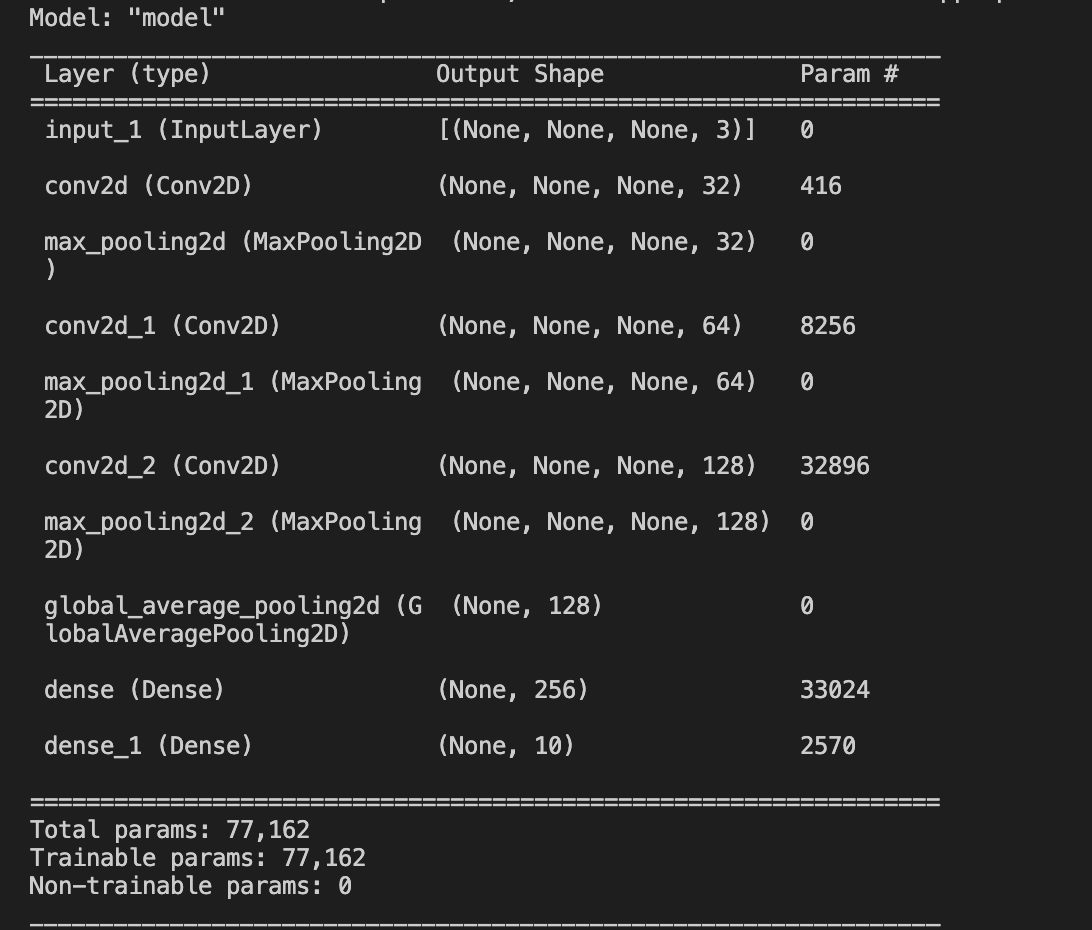
\includegraphics[width = \linewidth]{model_1_params.png}
		\caption{Smaller Model Summary}
	\endminipage\hfill
	\minipage{.49\textwidth}
		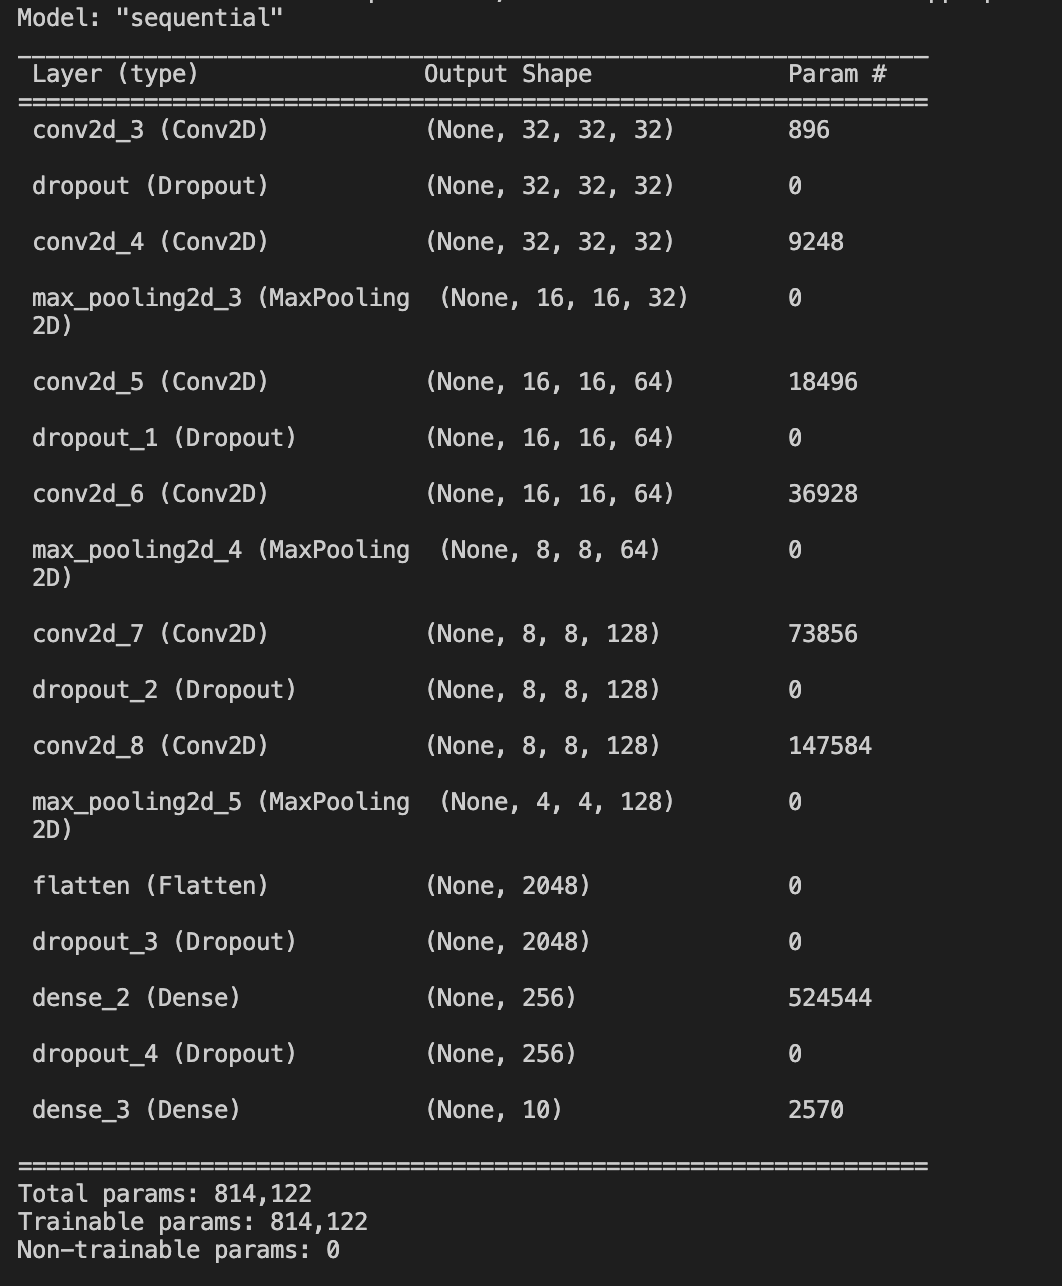
\includegraphics[width = \linewidth]{model_2_params.png}
		\caption{Larger Model Summary}
	\endminipage\hfill	
\end{figure}
\subsection{Dataset Creation}

To create the 6 (one for each compression that we are doing and the control dataset) different datasets that we need, we made use of python's numpy library that has an SVD function. Similar to the image compression problem in homework set 2, we separated each image by its red, green, and blue matrices and used SVD on each matrix. We then took the $n$ features that we wanted from the $U$ matrix that was generated by SVD and put the image back together. After the image was put back together, we add it to a list of images that will then be split up between training and testing. The labels are not changed in any way.

\subsection{Model Training}

To test the performance of our model architectures, we trained them using Clemson's Palmetto HPC. In total, we trained 12 models, a small and large model for each dataset that we created. For our hyperparameters, we trained for 200 epochs, a batch size of 32, and a learning rate of .001. Additionally, we chose to use the Adam optimizer, as it is very common and a gold standard for many model types in deep learning. We used keras' sparse cross-entropy loss for the multi-classification problem that we are faced with.

\section{Results}
\begin{figure}[!htb]
	\minipage{.49\textwidth}
		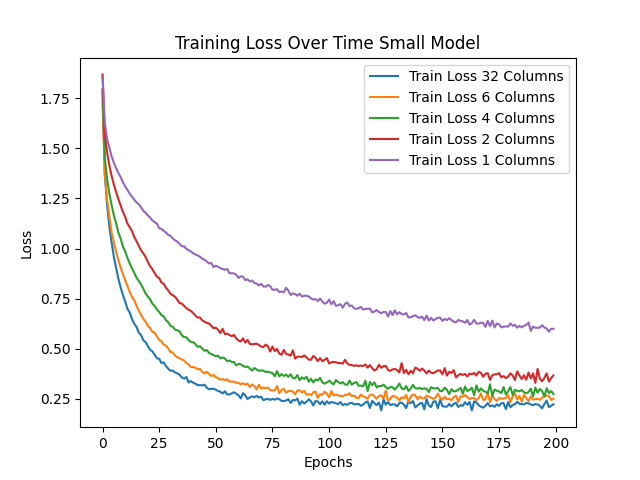
\includegraphics[width = \linewidth]{figures/train_loss_over_time_small.png}
		\caption{Smaller Model Training Loss}
	\endminipage\hfill
	\minipage{.49\textwidth}
		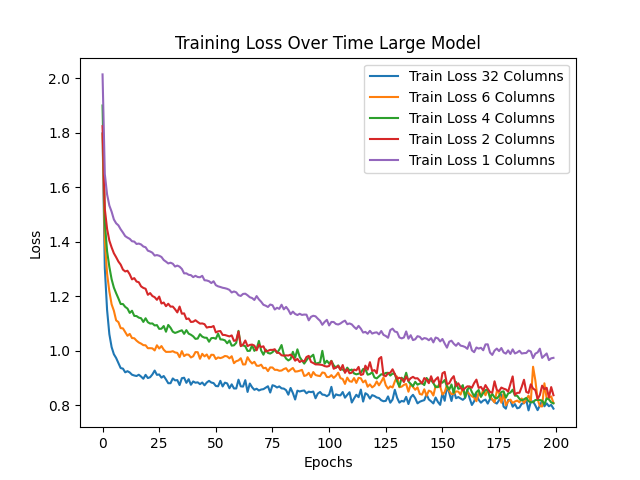
\includegraphics[width = \linewidth]{figures/loss_over_time_large_model.png}
		\caption{Larger Model Training Loss}
	\endminipage\hfill	
\end{figure}
\begin{figure}[!htb]
	\minipage{.49\textwidth}
		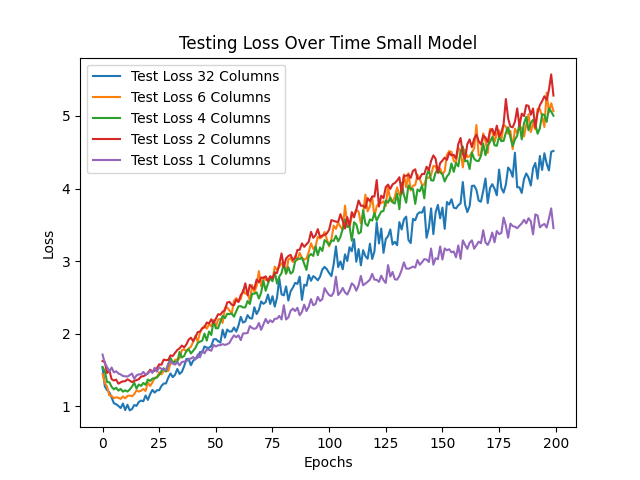
\includegraphics[width = \linewidth]{figures/test_loss_over_time_small.png}
		\caption{Smaller Model Validation Loss}
	\endminipage\hfill
	\minipage{.49\textwidth}
		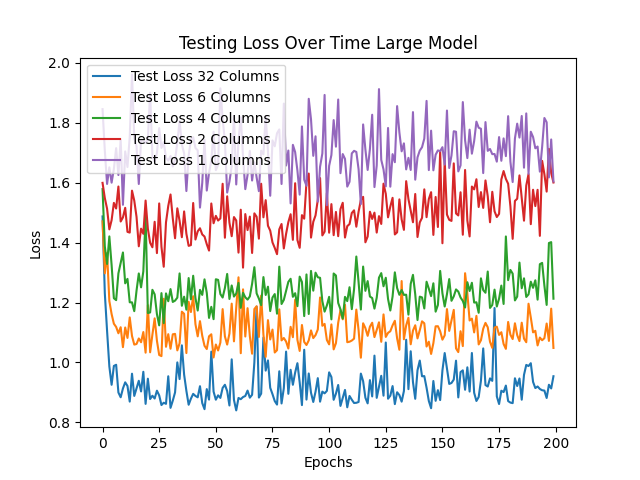
\includegraphics[width = \linewidth]{figures/test_loss_over_time_large_model.png}
		\caption{Larger Model Validation Loss}
	\endminipage\hfill	
\end{figure}
\begin{figure}[!htb]
	\minipage{.49\textwidth}
		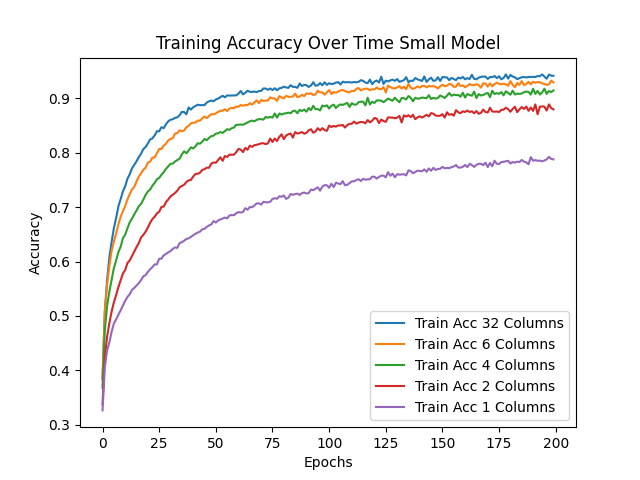
\includegraphics[width = \linewidth]{figures/train_acc_over_time_small.png}
		\caption{Smaller Model Training Accuracy}
	\endminipage\hfill
	\minipage{.49\textwidth}
		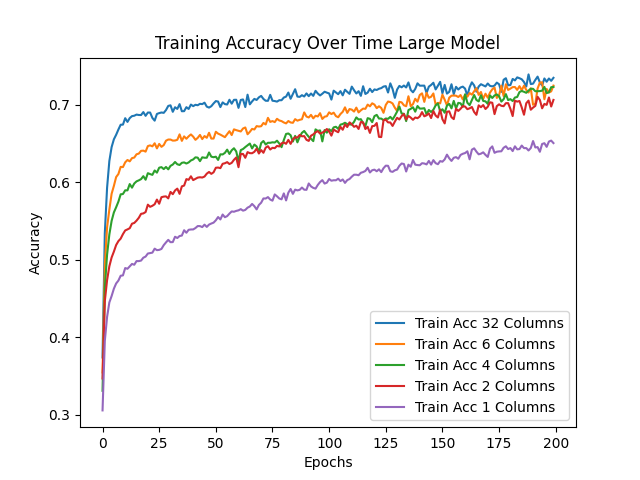
\includegraphics[width = \linewidth]{figures/train_acc_over_time_large_model.png}
		\caption{Larger Model Training Accuracy}
	\endminipage\hfill	
\end{figure}
\begin{figure}[!htb]
	\minipage{.49\textwidth}
		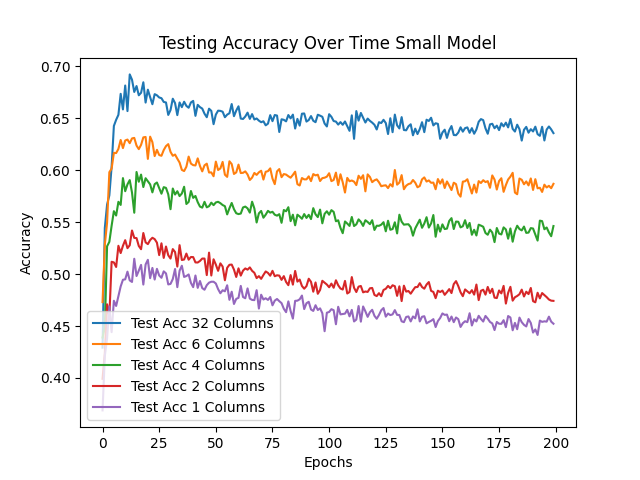
\includegraphics[width = \linewidth]{figures/test_acc_over_time_small.png}
		\caption{Smaller Model Validation Accuracy}
	\endminipage\hfill
	\minipage{.49\textwidth}
		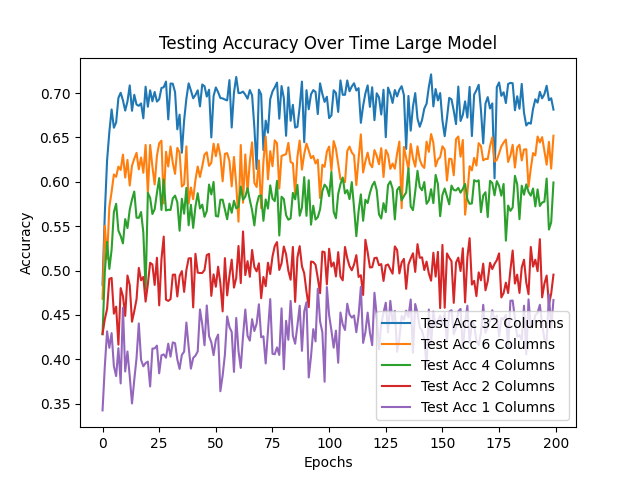
\includegraphics[width = \linewidth]{figures/test_acc_over_time_large_model.png}
		\caption{Larger Model Validation Accuracy}
	\endminipage\hfill	
\end{figure}

Based on our results, we confirm our hypothesis that the larger model performs better than the smaller model. As seen in the test loss for the small model, regardless of the amount of features utilized, there is a global minimum of loss and then the loss starts to diverge from the x-axis. The small model begins to overfit the data after about 15 epochs, and we learn that the small model might need to be trained for less time. The large model does not overfit the data, and we believe this to be the case because of the dropout layers in the architecture as well as the larger model most likely learning slower than the small model architecture. We also think that the larger model may need to be trained for longer due to a lack of convergence in the loss and accuracy. The testing loss in the larger model does not converge and smooth out at a certain epoch, so we believe that training longer might help with the convergence of the model. Another approach to help the convergence would be to lower the learning rate to a value such as .0001, so that the larger model learns even slower.
\end{document}